% Authorship: Claude-drafted, author-revised
\section{Weighing Does the Work}

Part VI left two questions standing, and the first has an answer that runs
in Berman's favor. The divergence among the four mechanisms is not an
artifact of his particular way of adding principles up. Rather than to Simple Additive Weighting's particular form, the property
that makes his rule the kind of rule it is belongs to a whole class of
rules. So Parts IV through VI established results about weighing
rather than results about one equation. That is
not to say the family is uniform in every respect. One line inside the
space of aggregation rules does decide cases, and it is not the line
between one weighted sum and another.

It is the line between a rule that
reads how strongly each principle applies and a rule that reads only
which way each one points.

The variation in this Part, and its limits, are worth stating before any
result, because the experiments here do not share one design. The magnitude
probe that sorts the ten rules, and the cardinal-ordinal disagreement grid
that follows it, both run across nine configurations at thirty seeds each:
three weight regimes, exactly equal, moderate, and high-variance, crossed with
three activation regimes, independent, category-correlated, and fully
correlated. One of those labels differs from Part III's, and one carries a second name
here. The equal regime sets every weight to the same value, where Part III's
uniform distribution draws near-equal ones. The high-variance regime is Part
III's own, and it is the one this Part also calls graded. The scores Figure~\ref{fig:f5-cardinal} draws are a single seeded
draw of three thousand cases at moderate weights on independent activations,
the configuration the rest of the Article uses, and the grid tests whether
they survive the other eight. The thirty-seed mean for that same cell differs
from the drawn figures by at most three thousandths. The closeness analysis
below is
a single battery of twenty thousand cases at one weight vector, and says so
where it is reported. The determinacy and verdict-agreement figures reported
across the ten rules come from a further battery of three thousand cases at
twenty seeds, run at the moderate weight distribution alone. None of this
carries the four mechanisms of Part VI
through the ten rules, and no claim here does.\footnote{Ten rules in three classes. \textit{Cardinal}: Simple
Additive Weighting gated at $\tau = 0.2$; SAW-sign, which decides on the
bare sign of net force; SAW-$L_1$, the normalized variant, which rescales
the weights to sum to one before adding; and the
nonlinear combination described in Part~III.B, in which a principle's
contribution grows faster than linearly in its activation.
\textit{Ordinal}: a bare vote-count, a weighted vote, a Borda count, and
a median-sign rule. \textit{Lexical}: lexicographic ordering and cascade.
The class labels record what each rule reads, not how well it performs.
Two of the ten are controls rather than independent rules: SAW-$L_1$ is
sign-identical to SAW-sign, since a positive rescaling of the weights
cannot change the sign of the sum, and is included only to forestall the
normalization objection; median-sign coincides with vote-count on a panel
of odd size. The four mechanisms of Part~VI are not carried through the
aggregation family, and this Part makes no claim that they were.}

The design still answers Part VI's question, in a narrow form that arguably
suffices, and the answer takes two steps rather than one. The property that
makes the family the family, sensitivity to how strongly a principle
applies, is met by every rule inside it and by no rule outside it. So the
results of Parts IV through VI would appear to be properties of weighing
rather than properties of Simple Additive Weighting. And every rule in that family computes each
principle's contribution as its weight multiplied by its activation, so a
change in the weights changes what the rule returns, directly and by
construction. That second step bears on Part VI, where the divergence
lives in the weights rather than in the activations: to blunt a
disagreement about weights, a rule would have to stop reading them.

By a single measurement, the magnitude probe, the rest of this Part sorts
that family. Inside the family Berman endorses the property survives every choice of
rule, so nothing in Parts IV through VI would appear to turn on the
particular equation. Across the line that
separates weighing from counting the choice is not idle at all. It decides
real cases, and the cases it decides are the close ones. After that, one
question remains, and it is Part VIII's: is any of this an artifact of the
determinacy threshold?

\subsection{Three Classes, One Measurement}

Berman writes down one rule for combining principles, but the rule
belongs to a family, and the family divides on a single question a judge
could be asked directly: when the principles conflict, does the rule read
how strongly each of them applies? There are three answers.

At one end, a \textit{cardinal} rule reads the magnitudes. Each principle contributes
force in proportion to how strongly it bears on the case, the forces are
summed, and the sign of the sum gives the verdict. A principle that barely applies contributes little. Three principles that
apply moderately can outweigh one that applies with full force. As written,
that is Berman's rule, and it is a family rather than a single equation. One can normalize the
forces to a fixed scale, decide on the bare sign rather than gate the
result at a threshold, or let a principle's contribution grow faster than linearly in how strongly
it applies, and still be reading magnitudes throughout.

In the middle, an \textit{ordinal} rule reads only which way each principle
points, and at most how the principles rank against one another within the case,
never how strongly any of them applies. The principles vote, and the
verdict goes to the side with more votes. A principle that barely applies
and a principle that applies overwhelmingly cast the same vote.

At the far end, a \textit{lexical} rule reads neither. The principles stand in a fixed
order of priority, the highest-ranked principle that speaks to the case
decides it, and everything below is silent, however strongly it applies
and however many principles are ranged on the other
side.\footnote{Berman, \textit{Practices}, \textit{supra} note 7, at
311--13, 333 (distinguishing genuine weighing from lexical priority and
placing principled positivism on the weighing side of that line).
Lexicographic ordering and cascade, and their associations with Raz's
exclusionary reasons and with categorical textualist orderings
respectively, are described in Part~III.B, \textit{supra}.}

The distance from the second of these to the third is not a further step
in the same direction. Throwing away the magnitudes, an ordinal rule keeps the plurality: every
principle still participates, and the many can still outvote the few. A
lexical rule throws away the plurality as well. One principle decides and
the rest are excluded. On Berman's picture both are required: a plurality
of principles and a magnitude for each. The
ordinal rules keep one of the two; the lexical rules drop both.

The three classes therefore stand in three different relations to the
theory, and it matters to keep them apart.

The lexical rules are a
\textit{foil}. Berman does not survey fixed priority among candidate structures for
principled positivism and set it aside because it performs badly. He
defines the theory against it. A rule of fixed priority is
not, then, a version of principled positivism that this Part puts to the
test. It is here for a narrower and, I think, more useful purpose. The
magnitude-weighing requirement of Part III asks that the weighted sum respond
to magnitude several times more than a rank-only rule does, and a
requirement of that form has no scale until something occupies the zero.
Run on the same cases, the lexical rules are what a rule that does not read
magnitude looks like. They are the calibration, and nothing much follows from their beating or
losing to the weighted sum on any other measure.

The ordinal rules are a \textit{rival}. Berman does not name them and reject them. Nothing in a legal system that
fixed content by a tally among principles would be incoherent, and
institutions decide by counting all the time.

The class is more than a plausible alternative: it is the nearest
neighbor to a position Berman himself allows. On this he is explicit: his account does not require the principles to
carry different weights. Give every principle the same weight and the weighted
sum begins to look like a count of which side more principles favor. It is not one, and Part IV proved that it is not, though the proof and the
figure are separate things. The proof establishes that the two rules disagree
on a set of positive measure. The measurement, with every weight equal, puts
the disagreement at about fifteen percent of cases, because the
sum reads the magnitudes the count discards. In that limiting case the whole distance between them is the
magnitude information.

That is arguably what makes ordinal aggregation the one genuine alternative
in this space. Except for the single property the magnitude-weighing
requirement credits, it keeps everything Berman's rule has, so the gap between the two
measures what that property is worth. The lexical
foil cannot do that job, because it differs from the weighted sum in two
ways at once, in magnitude and in plurality, and a comparison across two
differences localizes neither.\footnote{Berman, \textit{Practices},
\textit{supra} note 7, at 323--24 (the account does not require that the
principles carry varied weights). That equal weights do not collapse the weighted sum into a vote-count is
Theorem~5, \textit{supra} Part~IV.D, which proves the disagreement has
positive measure and supplies no rate. The $15.3\%$ figure reported below,
under equal weights and independent activations, is measured; it agrees with
the $15.4\%$ measured independently in Part~IV and serves as a check on this
Part's runs rather than as a new result.}

From those three roles the design of this Part follows. Whether the
results of Parts IV through VI depend on Simple Additive Weighting in
particular is a question answered inside the cardinal family, among cousins. What weighing magnitude is
worth is a question answered across the cardinal-ordinal line, against a rival. The lexical foil answers
neither question, and is not asked to.

An ordinal rule is not an exotic construction. It is what a court would seem to do whenever it asks which side has more of
the recognized considerations behind it and stops there. Voting is also how a multimember court settles
its own disagreements, so a theory that fixed legal content by a tally
among principles would be borrowing a familiar institutional form rather
than inventing one.

Here I run four versions of that tally. A bare
\textit{vote-count} gives each principle one vote. A \textit{weighted
vote} lets each principle's vote count in proportion to its standing, so
that the principles differ in authority but still cast votes rather than
exert forces. A \textit{Borda count} ranks the principles by how strongly
they apply within the case and then awards points by rank position alone,
so that the principle ranked first scores the same whether it barely
applied or applied overwhelmingly. And a \textit{median} rule takes the
middle vote and ignores the extremes.

Already used in Parts III and IV, the measurement that sorts the family is
the magnitude-only probe, and it is easiest to state as a case. Take a
dispute and hold fixed which principles bear on it, which way each of
them points, and how they rank against one another in force. Change only
how strongly each applies. In doctrinal terms the case is otherwise
identical: the same considerations are in play, the same ones favor each
side, they stand in the same order of force, but the dignity claim is now
somewhat weaker and the textual claim somewhat stronger. Then ask how
often the verdict changes. A rule that reads magnitudes can come out the
other way. A rule that reads only signs and ranks cannot, because nothing
it consults has moved.\footnote{The probe perturbs only the magnitudes of
the activations, holding every sign and every within-case rank fixed, and
reports the share of cases whose verdict changes; see \textit{supra}
Part~III.C and Part~IV.C. The scores are: SAW at $\tau = 0.2$, $0.0496$;
SAW-sign, $0.0229$; SAW-$L_1$, $0.0229$; nonlinear, $0.0749$; all four
ordinal rules, $0.000$; lexicographic, $0.0024$; cascade, $0.000$.
Part~IV reported the weighted sum's magnitude sensitivity as $0.0256$
against a lexical rule's $0.0026$, a ratio near ten; the comparable
figures here are $0.0229$ against $0.0024$, a ratio of $9.75$. The ratio
is stable across the two runs and the level moves with the gate, because
a gated rule can also be pushed across the determinacy threshold by a
magnitude-only change, so that a flip between determinate and
indeterminate counts as a verdict change. That is why the gated weighted
sum scores $0.0496$ here and the ungated bare-sign rule $0.0229$, and why
Part~IV used the ungated figure. Where a ratio is at issue this Article
reports it as about ten times, which both runs support.}

Run across the ten rules, the probe sorts them by class. On between $2.3\%$ and $7.5\%$ of cases the four cardinal rules change
their verdicts, with Berman's own rule, gated at $\tau = 0.2$, at $4.96\%$. Every ordinal rule changes its verdict on exactly none of them, a flat
$0.000$, as one would expect of a rule that never reads a magnitude.
The lexical rules sit within rounding of the same zero, $0.24\%$ for
lexicographic ordering and $0.000$ for cascade.
Figure~\ref{fig:f5-cardinal} shows the ten side by side.

Those scores come from a single configuration, so the question they leave
open is whether the class separation is a fact about the rules or an
artifact of where it was measured. Run across all nine configurations at
thirty seeds each, the answer divides. The separation would seem robust to the weights and fragile to the
activations.

How the weights are distributed turns out to be idle. Moving from exactly
equal weights to moderate to high-variance barely moves any rule's score,
the rough-weights finding of Part IV showing up again in a
different measurement. How the activations are structured is not idle at
all. The ordering survives correlation and the margin does not. On independent
activations the lowest cardinal score clears the highest non-cardinal score by
about ten to one; under the category correlation of realistic cases the
ordering holds but the ratio falls to about four to one, below Part III's
five-fold bar. Under full correlation the ordering itself fails: the lowest
cardinal score drops to the lexical foil's level.

All three of those ratios are computed on the ungated rule, and the
requirement is not scored on it. Scored where Part III scores it, on the gated weighted
sum, the bar clears comfortably on independent activations and clears under
category correlation as well, and fails only under full
correlation.\footnote{Thirty seeds in each of nine configurations. Ratio of
the lowest cardinal score to the highest non-cardinal score: independent
$9.58$ to $9.80$, category-correlated $4.05$ to $4.42$, fully correlated
$0.86$ to $0.97$, across the three weight regimes. Taking the gated weighted
sum instead, which is the rule the requirement is scored on, the corresponding
ratios are $18.9$ to $19.4$, $8.2$ to $8.6$, and $1.8$ to $1.9$. So the
requirement clears its bar on the independent and the category-correlated
activations alike, the two structures short of full correlation, and the
four-to-one figure is a property of the ungated comparison.}

That failure is a property of the cases rather than of the rules, and
saying which matters. When every principle fires together there is almost
no magnitude-only variation left for the probe to move, so a rule that
reads magnitudes has nothing to read and scores like a rule that does not.
Full correlation is arguably the far end of the range tested here, and it
is not the structure this Article calls realistic. But the requirement should be
understood accordingly: the weighted sum weighs magnitude where the cases
still contain conflict, which is where the theory's question arises at all,
rather than in every possible arrangement of the facts.

\begin{figure}[t]
\centering
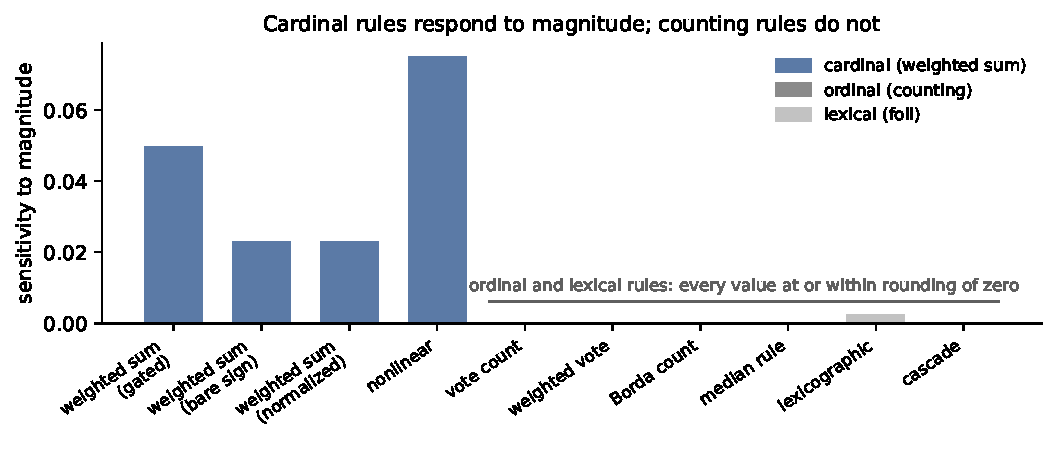
\includegraphics[width=\textwidth]{F5_cardinal_ordinal}
\caption{Only cardinal aggregation reads how strongly a principle
applies. Under a magnitude-only perturbation, which holds every sign and
every within-case rank fixed and changes only the strengths, the four
cardinal rules change their verdicts on $2.3\%$ to $7.5\%$ of cases;
Berman's weighted sum sits at $4.96\%$ with its determinacy gate at
$\tau = 0.2$ and at $2.3\%$ on the bare sign of net force, which is the
clean cardinal reference, the gap between the two being the cases the
gate moves across the determinacy threshold rather than across the verdict.
Every ordinal counting rule changes its verdict on exactly none of them
($0.000$, by construction, having never read a magnitude), and the
lexical foils on effectively none (lexicographic $0.24\%$, cascade
$0.000$). The measurement separates the cardinal family from the other
six rules by roughly a factor of ten at its narrowest. It does not
separate the ordinal rival from the lexical foil, which sit together at
or within rounding of zero; that division is a conceptual one about what
each rule does with the principles it declines to weigh, not one this
instrument reports. Only the cardinal family is faithful to Berman's
picture of principles that weigh rather than rank.}
\label{fig:f5-cardinal}
\end{figure}

Half of that result is definitional, and Part IV said as much of the
lexical comparison. The point extends to the ordinal class. That a rule
which reads only signs and ranks scores zero under a probe that moves
only magnitudes is not a rounding and not a finding. It is what such a
rule does, by construction, when a magnitude changes. The non-definitional
half is that every rule in the cardinal family responds
substantially, at rates from two to seven percent where the ceiling on
the entire far side is a quarter of one percent, and the requirement credits
exactly that.

The second caveat concerns what the probe does not show. By a factor of about ten at its narrowest, the cut it makes is between the
cardinal rules and everything else. It does not separate the ordinal rules from the
lexical ones, and it is not asked to. On this measurement the two are
alike, both at or within rounding of zero, and lexicographic ordering is
if anything marginally the higher of the two. Into a rival and a foil, the division of that far side is a conceptual one,
resting on what each rule does with the principles it declines to weigh and
on how each stands toward the theory, not a division this instrument
reports. The figure shows exactly that: four bars with height and six lying on the
axis. No more should be read off it.

\subsection{Inside the Weighing Family, the Form Is Idle}

The property that makes the family the family, sensitivity to how
strongly a principle applies, is met by every cardinal rule tested and by
no ordinal or lexical rule. That is a narrower claim than it may look, and the narrowness is
deliberate. Only one of Part III's four requirements is measured rule by
rule here. Well-definedness is a property of the weight vector rather than
of the aggregation rule, and by construction it is constant across all ten. For the weighted sum alone, noise tolerance and the margin over the
hierarchical Hart are measured, and for a reason given below they could not
be measured like-for-like across the whole set in any event. But the requirement that carries Berman's
distinctive commitment is exactly the one the probe measures, and it
comes out as a property of the class rather than an artifact of Simple
Additive Weighting's functional form.

In this battery the weighted sum's own reference figure is a determinacy
margin of $+0.268$ over the hierarchical Hart, the charitable comparator of Part IV. It sits with the margins already on the record: $+0.272$
for the stipulated engine in Part IV, and the mechanism cluster of Part
VI, uptake near $0.27$, reliance $0.291$, strategic $0.283$, appointment
$0.284$. Nothing in this Part's battery moves it.

Of the two comparisons the battery supplies, one has to be set aside, and
setting it aside is the methodological point on which the rest of this
Section depends. A \textit{gated} rule holds a threshold below which it
declines to decide and reports the case as unresolved. An \textit{ungated}
rule has no such threshold. As run here the weighted sum is gated: at $\tau = 0.2$ it decides $86.3\%$
of cases and reports the remaining $13.7\%$ as unresolved. Every other rule
in the set is ungated, so it converts every case into a verdict, breaking
ties by whatever its construction supplies, and posts a determinacy rate of
$1.000$ (Borda alone falls short, at $0.996$, and its shortfall is exact
rank ties). That is not more law. It is the same law with the cases in
equipoise relabeled as decided.

That inflation is easy to quantify. Of these same cases the hierarchical
Hart decides $59.4\%$. Against it the ungated rules show an apparent
determinacy margin of $+0.406$ where the weighted sum's margin is
$+0.268$, and the extra fourteen points are bought entirely by never
abstaining.

What makes this a methodological correction rather than a defense of
Berman's rule is where the inflation lands. On the faithful members of the
cardinal family it falls exactly as it falls on the foils.
The sign variant and the normalized variant of the weighted sum both post
$1.000$ for precisely the reason lexicographic ordering and cascade do,
and the sign variant is the bare-sign rule that Part III takes as the
faithful baseline and that Berman himself endorses. On continuously distributed activations exact equipoise has probability
zero, so Berman's own preferred rule never abstains and posts a perfect
determinacy rate for no substantive reason at all. Across a gated and an
ungated rule, therefore, no determinacy figure and no margin over the
hierarchical Hart is like-for-like, and none is offered here as though it
were.\footnote{That the bare sign of net force is Berman's own faithful
baseline is \textit{supra} Part~III.A; see Berman, \textit{Practices},
\textit{supra} note 7, at 331 (an aggregative system ``could incorporate
thresholds or eschew them'').}

The second comparison the battery supplies is verdict agreement, the share
of cases on which each rule returns the weighted sum's own verdict, and it
carries a ceiling that has to be stated before the figures can be read at
all. At $0.863$, the bare-sign variant's raw agreement is numerically
identical to the weighted sum's own determinacy rate, and the identity is
not a coincidence. The weighted sum abstains
on $13.7\%$ of cases and no ungated rule ever abstains, so no ungated
rule can exceed $0.863$ on the raw measure.

Restricted to the cases the
weighted sum actually decides, the sign variant and the normalized
variant return its verdict on all of them. Read raw, the figures invite
the inference that the sign variant \textit{only} agrees with the
weighted sum six times in seven, when in fact it never once departs from
it where the weighted sum speaks.

Read on the cases the weighted sum decides, the figures also contain a
result that does not favor this Part's thesis, and it belongs in the text
rather than in a footnote. Agreement does not track class membership. By
far the most distant are the lexical foils, returning the weighted sum's
verdict on $0.668$ and $0.650$ of the cases it decides, and the theory would
predict exactly that of the thing it defines itself against. But the nonlinear
rule, a faithful cardinal member of the family, agrees on $0.881$, below
every ordinal rule in the set (vote-count and the weighted vote
at $0.886$, Borda at $0.921$).

Properly normalized, the nonlinear rule is the most distant from the
weighted sum of the six distinct in-theory rules, setting the two controls
aside. This Part's claim is therefore about the requirement and about the
class separation the magnitude probe reports. It is not a claim that the
cardinal family is uniformly closer to the weighted sum on verdicts,
because it is not, and this Part does not treat verdict agreement as a
measure of fidelity to the theory.\footnote{Share of cases on which each
rule returns the weighted sum's verdict: SAW-sign $0.863$, SAW-$L_1$
$0.863$, nonlinear $0.761$, vote-count $0.765$, weighted vote $0.765$,
Borda $0.795$, median-sign $0.765$, lexicographic $0.577$, cascade
$0.561$. These raw shares carry a ceiling: the weighted sum abstains on
$13.7\%$ of cases and no ungated rule ever abstains, so no ungated rule
can exceed $0.863$, and SAW-sign reaches it exactly. Restricted to the
cases the weighted sum decides, the shares are SAW-sign and SAW-$L_1$
$1.000$, Borda $0.921$, weighted vote $0.886$, vote-count and median-sign
$0.886$, nonlinear $0.881$, lexicographic $0.668$, cascade $0.650$.}

Two of the ten labels are controls rather than independent evidence, and
saying so keeps the count honest. By construction the normalized variant is
sign-identical to the sign variant, since a positive rescaling of the
weights cannot change the sign of a sum; it is included only to forestall the objection that the result
depends on the scale of the weights. And the median rule coincides with
the bare vote-count on a panel of odd size. Ten labels are eight distinct
verdict rules.

What this Section establishes, then, is that the results of Parts IV
through VI do not rest on Simple Additive Weighting rather than on some
cousin of it. On the linear form Berman's picture does not appear to stand
or fall:
the property the theory is defined by belongs to every rule in the
family, and the normalization and gating variants of his own rule return
his verdict on every case he decides. The scope limit stated at the
outset holds here too. This is established for the defining property and
for these cases. It is not established by running the four mechanisms of Part VI through ten
aggregation rules, which this Part did not do, and a design that did might
well report otherwise.

\subsection{The Disagreements Sit in the Close Cases}

Because both sides of it can be made ungated, the comparison across the
cardinal-ordinal line is the cleanest measurement in this Part. On the
cardinal side here is the bare-sign rule rather than the gated weighted
sum, chosen so that both rules decide every case and the gate cannot
contaminate the contrast. The ordinal side is the counting family.

With every principle carrying exactly equal weight and activations drawn
independently, the two disagree on $15.3\%$ of cases. The equality has to
be exact rather than near, because that is the condition Theorem 5 is
stated under. Part IV measures the same quantity at $15.4\%$ on a separate implementation.
Two independent batteries landing within a tenth of a point is a check on
both, and it is the only check available, since Theorem 5 establishes that the
disagreement is nonzero without fixing how large it is. It is worth being
clear about what the number is not. It is not a claim that either rule is right, and nothing in the design
would support one. It is the share of cases on which the choice between reading magnitudes and
counting votes appears to change the verdict. Berman, shown an early
version of this comparison, called the cardinal-ordinal finding striking,
and added that he had nothing to say about it yet.\footnote{E-mail from
Mitchell N.\ Berman to author (Mar.\ 2026) (on file with author)
(describing ``the finding regarding cardinal aggregation vs ordinal
ranking'' as ``striking'' and as ``interesting and surprising''). The
reaction is to the contrast between weighing and counting, not to the
particular rate reported here.}

With the structure of the cases the rate moves, and one of the two trends
looks robust. As the activations become correlated, the disagreement falls,
and it falls in all nine combinations of ordinal rule and weight
distribution without exception. From $15.3\%$ under independent
activations, the counting rules fall to between $11.5\%$ and $12.2\%$
under the category correlation of realistic cases, in which principles of
the same category tend to fire together, and to $2.9\%$ under full
correlation, where every ordinal rule ends between $1.4\%$ and $3.2\%$.
(Borda runs lower under category correlation, at $5.6\%$ under graded weights
and $7.3\%$ under moderate ones, so the eleven-to-twelve figure is the
counting rules alone. Its equal-weights cell is set aside for the reason given
below.) The fall itself holds for every rule and every weight regime,
including the cells that are set aside, since what contaminates those is
constant across the activation axis along which the fall is measured. The reading is straightforward enough. When a category of principles fires
as a bloc, the side carrying the greater force is generally also the side
with the greater number, and counting and weighing point the same way.

The second trend is weaker and should be reported as such. As the weights
spread out, the counting rules disagree with the bare-sign rule slightly more
often: the bare vote-count runs from $15.3\%$ under equal weights to $15.8\%$
under moderate weights and $17.8\%$ under graded ones, and the weighted vote
from $15.3\%$ to $15.8\%$ to $16.4\%$. Those are movements of two and a half
points and one, across the whole span of weight dispersion the Article tests.

The Borda rule is not reported here, because its equal-weights cell does not
measure what the label says. The implementation converts the weights to their
ranks before scoring, and a vector of identical weights has no ranks to
convert, so the procedure supplies an arbitrary ordering of the nine
principles in whatever sequence they are stored. Under graded weights the
conversion is meaningful and the cell is sound; under exactly equal weights it
is not, and no trend that uses that cell as an endpoint can be
read.\footnote{The defect is confined to this comparison. Borda's
magnitude-probe score is exactly zero in every configuration, which is what
the class separation uses it for, and the ranking it is handed does not affect
a probe that holds ranks fixed.} So the direction in which weight dispersion
moves the cardinal-ordinal gap is reported for the counting rules alone, and
no general law about ordinal aggregation should be read off it.

One convention from Part IV has to be suspended here rather than carried
forward. As the conservative baseline, Part IV banked independent
activations and asked that every figure be read as a floor, because
correlation improves the model's performance. That convention is about the
model's performance, and this quantity is not a performance measure.
For the cardinal-ordinal disagreement rate the convention runs the other
way. Independent activations produce the largest gap, presumably because
principles firing independently produce the close cases where
counting and weighing part company. Along the correlation axis the $15.3\%$ is an upper bound
on this quantity rather than a floor, and the figure for realistic cases
is the middle band.
Carried forward, Part IV's convention would likely lead a reader to misread
the headline in this Article's favor.\footnote{The fall with correlation is monotone
across every rule and weight regime tested, so Part~IV's floor convention
does not carry over to this measurement.}

One further feature of the grid licenses a claim that would otherwise be
rhetorical. In all nine cells, for the bare vote-count and the weighted
vote, the disagreement rate and the opposite-verdict rate are identical to
the last digit. Both rules are ungated, and so is the cardinal
rule on the other side, so every disagreement is a case in which each
rule reaches a verdict and the two verdicts point opposite ways. These are flat contradictions, not cases in which one rule decides and the
other falls silent. Among the four, Borda is the small exception,
abstaining on exact rank ties in about four cases in a thousand.

Where those contradictions sit in the run of cases is perhaps the sharpest
result in this Part. At issue is the size of the net force introduced in Part
II, the balance the weighted sum computes, positive for one side and negative
for the other, so that its size measures how far the case is
from a tie: a large net force is a lopsided case, and a net force near
zero is a case in near-equipoise.

Sort a battery of twenty thousand cases by that quantity and the
disagreements collapse into the closest ones. On the cases where the two
rules disagree the mean size of the net force is $0.35$, against $1.03$
where they agree. On the closer half of the caseload the disagreement rate
is $29.9\%$, against $2.9\%$ on the farther half, and $91.1\%$ of all the
disagreements fall in the closer half. The most
direct statement of the result needs no grouping at all: across those
twenty thousand cases, the largest net force on which the two rules
disagreed anywhere was $1.61$, against an observed maximum of $4.44$.
Nineteen percent of the cases carry a net force above $1.5$, and exactly
four of them are disagreements.

Cut the same sorted caseload into ten equal groups, deciles, the first
holding the closest tenth of cases and the last the most lopsided tenth,
and the profile is the one in Table~\ref{tab:closeness}. Steep as the gradient is, it is a gradient and not a wall: the rate is
still $15.2\%$ at the median case, and only the most lopsided tenth is
exactly zero.

\begin{table}[t]
\centering
\small
\caption{Disagreement concentrates in the closest cases. Equal-count
deciles of the caseload, sorted by the size of the net force.}
\label{tab:closeness}
\begin{tabular}{lc}
\toprule
\textbf{Decile of cases, by net-force size} & \textbf{Disagreement rate} \\
\midrule
1 (closest cases)  & $44.9\%$ \\
2                  & $39.0\%$ \\
3                  & $30.2\%$ \\
4                  & $20.4\%$ \\
5                  & $15.2\%$ \\
6                  & $8.0\%$ \\
7                  & $4.8\%$ \\
8                  & $1.6\%$ \\
9                  & $0.3\%$ \\
10 (most lopsided) & $0.0\%$ \\
\bottomrule
\end{tabular}
\end{table}

That interpretation is the payoff of the Part. When the principles on one
side plainly outweigh those on the other, counting and weighing return the
same verdict, because the side carrying the greater force is generally also
the side with more principles behind it. On those cases magnitude
information is idle and the two rules are interchangeable. It becomes
decisive exactly where the case is close, and that is where a theory of legal content
is under the most pressure to supply an answer at all.

Behind that pattern lies a strongly activated minority of principles
outweighing a weakly activated majority. The sum finds for the minority,
the count finds for the majority, and because both rules decide, the two
contradict one another rather than one of them falling silent. Of that
description the minority half is analytic rather than merely observed. The panel holds
nine principles and exactly zero activations have probability zero, so a
vote-count always finds for a side holding at least five; whenever the
weighted sum disagrees with it, the sum is finding for a side holding
four or fewer. The magnitude half is measured. Where the two rules disagree, the losing
side carries $0.437$ of the total weighted force, against $0.324$ where
they agree. The disagreements would seem to be the cases in which the side
that loses is nearly as strongly supported as the side that wins.

Two limits attach to the result. The zeros are finite-sample zeros and not
entailments. Easy enough to construct is a lopsided case on which the two
rules disagree: five principles activated at $-0.1$ against four activated
at $+1.0$ yields a vote-count that finds negative against a large positive
net force. The observation is that across twenty thousand cases drawn from
nine independent activations none arose above a net force of $1.61$, not
that none can. And rather than the thirty-seed averaging used elsewhere in this Article,
this experiment is a single battery, one seed and one weight vector over
twenty thousand cases. Its overall disagreement rate
of $16.4\%$ is consistent with the thirty-seed grid's $15.8\%$ for the
matched configuration, which is the check available, but the figures
should be read as one battery's.\footnote{The cardinal side of this
comparison is the ungated bare-sign rule, so that both sides decide every
case and the gate cannot contaminate the contrast; cases are sorted by
the size of the net force the weighted sum computes. The figures come from
a single battery of twenty thousand cases at one weight vector rather than
from the thirty-seed averaging used elsewhere in this Article; its overall
disagreement rate of $16.4\%$ is consistent with the thirty-seed grid's
$15.8\%$ for the matched configuration.}

That concentration is arguably what vindicates the magnitude-weighing
requirement, and it supplies the half of the case that Parts III and IV
both flagged as missing. Their caveat was that half of the requirement's
evidence is definitional, since a rank-only rule is blind to a
magnitude-only probe by construction. The concentration supplies the
non-definitional half. The cases on which the blindness matters are the
close ones. On this showing, reading magnitude is not a decorative property
of Berman's rule. It decides
cases, and it decides the hard ones.

What follows is narrower than it may seem, and the narrowness is not a
hedge. Nothing here shows that cardinal aggregation is more
\textit{accurate} in close cases, because the design contains no ground
truth against which either rule could be scored, and this Part is not a
tournament with a winner. Nor does anything here show that ordinal rules are unreliable in any
general sense: on the cases the weighted sum decides they return its
verdict more than four times in five, and on the most lopsided tenth of
this battery they returned it every time. The claim is the narrower one: that the two differ, where they differ, and,
plausibly, why.

\subsection{What This Part Establishes}

Part VI's first question has an answer, and it runs in Berman's favor, though
the answer is narrower than the question. No rule inside the family Berman
endorses is indifferent to the weights, because every member computes each
principle's contribution as its weight multiplied by its activation, so the
weights the mechanisms disagree about enter the verdict directly. The
divergence cannot therefore be made to vanish by choosing a different rule
inside the family.

What is not established is that its rate would be the same under every such
rule. A rule can read the weights and still compress large differences among
them, and this Part did not run the four mechanisms through the ten rules. The
claim is that no member of the family dissolves the divergence, not that every
member reproduces it at Part VI's rate.

Of the whole set, only the unweighted vote-count and the median rule
discard the weights outright. Either would collapse the divergence to
nothing, but only by ignoring the weights altogether, which would abandon
the weighting the theory makes central rather than repair anything. That much is argument rather than measurement.
What is measured is that the defining property belongs to every rule inside
the family, at rates from $0.023$ to $0.075$, and to no rule outside it,
where the ceiling is $0.0024$, and that the separation survives every
weight regime and every activation structure short of full correlation, and that the normalization and
gating variants of Berman's own rule return his verdict on every case he
decides. Parts IV through VI are results about weighing, not results
about Simple Additive Weighting.\footnote{The stronger claim, that the
four mechanisms were carried through the aggregation family and the
divergence survived, is not tested here and is not made. What is
established is the narrower and sufficient claim in the text.}

The second thing this Part establishes concerns the commitment itself. The
one measurement that sorts the family is the measurement the theory is
defined by, the cardinal family sits alone on the weighing side of it, and
the line shows up in verdicts. On that evidence Berman's commitment to
weighing rather than ranking is doing work in his theory that it would not
be doing if the family were interchangeable across that line. It is not interchangeable.

Five limits travel with those conclusions, and collecting them in one place
is better than scattering them. This Part did not cross the four mechanisms
of Part VI with the ten aggregation rules. What it varied was the rule,
against three weight regimes and three activation regimes.

The determinacy figures and the margins over the hierarchical Hart are
not comparable across a gated and an ungated rule, so no such comparison
is offered, and the near-perfect determinacy of the ungated rules is an
artifact of never abstaining rather than a property worth having. The
magnitude probe separates the cardinal family from the other six rules
but does not separate the rival from the foil; that division rests on
what each rule does with the principles it declines to weigh, and this
instrument does not report it. The direction in which spreading the weights moves the cardinal-ordinal
disagreement rate depends on whether the ordinal rule counts or ranks, so
neither direction is a law. And the ordering that separates the classes holds
on independent and category-correlated activations but not under full
correlation, where a magnitude probe has almost nothing left to move. Part
III's five-fold bar is a stronger condition than that ordering, and on the
gated rule that the requirement is scored on, it clears the bar wherever the
ordering holds.

The one comparison this Part had to decline points to what comes next.
Because the weighted sum at $\tau = 0.2$ is the only gated rule in the set,
the determinacy comparison was unavailable, and what makes it the only
gated rule is the threshold. Part VI closed with two questions, and
this Part answers the first. What the choice of rule does control is
whether magnitude is read at all, and that controls real verdicts,
concentrated in the close cases. The second question is whether the
divergence, and the determinacy rates that carry it, are instead
artifacts of the determinacy threshold, the line at which net force
becomes a verdict. That is Part VIII's, and it is likely the last of the modeling choices that
could carry the result.
